%% Overleaf version: compiles on its own (pdfLaTeX, no BibTeX). GENERATED by manuscript/make_overleaf.py
\documentclass[journal=jctcce,manuscript=article]{achemso}
\usepackage[T1]{fontenc}
\usepackage{amsmath}
\usepackage{amssymb}
\usepackage{booktabs}
\usepackage{graphicx}
\usepackage{float}
\usepackage{placeins}
\usepackage[colorlinks=true,linkcolor=blue,citecolor=blue,urlcolor=blue]{hyperref}
\setkeys{acs}{articletitle=true,doi=true}
\DeclareMathOperator{\arcosh}{arcosh}
\DeclareMathOperator{\clip}{clip}

% All numbers in tables are \input from files written by the scripts in ../dc_scan and
% ../exact_vs_proposed (see ../README.md); build with ./build.sh.

\title{Probing Dimensional Crossover in SCAN Exchange with Exact Quasi-One-Dimensional Wires and Quasi-Two-Dimensional Sheets}

\author{Gabriel Chirchir}
\email{gabrielchirchir@gmail.com}
\author{Subrata Jana}
\author{Szymon \'Smiga}
\email{szsmiga@fizyka.umk.pl}
\affiliation{Institute of Physics, Faculty of Physics, Astronomy and Informatics,
Nicolaus Copernicus University in Toru\'n, ul.~Grudzi\c{a}dzka~5, 87-100 Toru\'n, Poland}

\keywords{SCAN, meta-GGA, density Hessian, dimensional crossover, quasi-one-dimensional, quasi-two-dimensional, exact exchange}

\hyphenation{an-iso-trop-ic an-iso-trop-ic-al-ly}
\usepackage{xcolor}
% new-result highlighting (user 2026-11-05): \novelty{...} prints red; for the final
% submission change {red} to {black} here (one line) to remove all highlighting
\newcommand{\novelty}[1]{{\color{red}#1}}
% Figures: names are unique to this paper (scan1d2d_*.pdf). Overleaf compiles from the project root, so if
% this folder sits inside a larger Overleaf project under a name not listed here, add {<folder>/figures/}.
\graphicspath{{figures/}{overleaf/figures/}{scan/figures/}{SCAN_1D_2D/figures/}{scan_1d_2d/figures/}{dcscan/figures/}{DC-SCAN/figures/}{scan1d2d/figures/}}
\begin{document}

\begin{abstract}
Recent work by Constantin, ``Dimensional crossover of the exchange-correlation
energy at the semilocal level,'' \novelty{Phys.\ Rev.\ B 78, 155106 (2008), DOI:
10.1103/PhysRevB.78.155106}, motivates our dimensional-crossover extension of SCAN
exchange.  That work showed that a semilocal functional can recover the exact
two-dimensional exchange limit if its enhancement factor decays as $s^{-1/2}$.
SCAN has a single tail of this kind and cannot use it selectively: on one-orbital
densities its iso-orbital indicator vanishes, so it cannot tell a sheet from a
wire and misses the exact exchange limits of both.  In this study, we address this
failure.  We have developed an exact fixed-density benchmark: two-electron
anisotropic Gaussian densities from the aniGTO harmonic-trap basis, whose exact
exchange is a single anisotropic repulsion integral evaluated in aniGTO.  Our
analysis shows that on this benchmark SCAN exchange grows as $\lambda^{1/2}$ on the
wire ($-292$~Ha against the exact $-7.90$~Ha at $\lambda=10^4$) and tends to
$-11.145$~Ha on the sheet, 8.9 times the exact limit $-\sqrt{\pi/2}$.  As a
solution, we propose DC-SCAN, which adds the log-density curvature through a rank
descriptor and a curvature scale, with two coefficients fixed analytically rather
than fitted.  DC-SCAN removes the power-law divergence, reproduces the exact
coefficient of the wire logarithm up to a constant finite-width offset of
$-0.040$~Ha, stays within 0.10~Ha of the exact sheet exchange and reaches its
limit, and leaves SCAN unchanged for isotropic and slowly varying densities.
\novelty{Applied to the infinite-barrier slab, our sheet construction reproduces
Constantin's coefficient (0.5217) and the SCAN two-dimensional limit of Kaplan,
Wagle and Perdew ($-1.671$~Ha) to 0.02\%, and we extend the analysis to the wire
limit, which has not been examined for SCAN against an exact reference.}  We keep
the benchmark exact at extreme anisotropy with a logarithmic-variable repulsion
integral, accurate to double precision where the default quadrature fails by up to
11.3~Ha, and an exact axisymmetric $N=2$ strictly-correlated solver.  These
fixed-density, exchange-only results are the basis for tests on non-Gaussian
profiles, three-dimensional norms, the self-consistent potential and correlation.
\end{abstract}

\section{Introduction}
\label{sec:intro}
Semilocal meta-generalized-gradient approximations (meta-GGAs) such as
SCAN\cite{sun2015strongly} are constructed for three-dimensional (3D)
densities.  In confined systems --- quantum wells, wires, monolayers and
anisotropic traps --- the density can be compressed along one or two axes, and
the exchange energy then follows a different asymptotic law: it stays finite
when one coordinate is compressed and diverges logarithmically when two are,
because the electrons still interact through the 3D Coulomb potential.
\novelty{Constantin showed that a semilocal functional recovers the exact two-dimensional
(2D) exchange of an infinite-barrier slab if its enhancement factor tends to
$0.5217\,s^{-1/2}$\cite{constantin2008dimensional}, and Kaplan, Wagle and Perdew
found that SCAN, alone among LDA, PBE and SCAN, reaches a finite 2D limit for this
slab, but one about an order of magnitude too negative\cite{kaplan2018collapse}.}
Semilocal exchange functionals collapsing from three to two dimensions have
been constructed\cite{horowitz2023collapsing}, and density-Hessian (Hessian-level)
meta-GGAs have been implemented self-consistently\cite{dabbaghi2026hessian}.
In this study, we address a narrower question: does SCAN exchange obey the two
confinement limits on solvable densities, and what is the lowest additional
density-derivative information needed to make it do so?

As test densities, we use two-electron densities generated by one doubly
occupied anisotropic Gaussian.  They are the simplest objects of the aniGTO
anisotropic Gaussian integral package\cite{chirchir2026anigto}: the orbital is
the $s$ function of the aniGTO harmonic-trap basis, and the exact exchange
energy is one anisotropic two-electron repulsion integral.  Because the
density is one-orbital, the SCAN iso-orbital indicator is $\alpha=0$
everywhere for every confinement strength, so $\alpha$ carries no geometric
information: a sphere, a sheet and a wire look the same to SCAN.  Whether SCAN
nevertheless respects the sheet and wire limits has not been checked against
exact references.  We show that SCAN then has the wrong asymptotic power on the
wire and the wrong finite limit on the sheet.  We then propose and test a
dimensional-crossover extension of SCAN exchange (DC-SCAN) that uses the
log-density curvature to select a sheet branch, a wire branch or unmodified
SCAN.  \novelty{Our sheet construction reproduces both slab results of
refs~\citenum{constantin2008dimensional,kaplan2018collapse} independently, and we
extend the analysis to the two-axis (wire) limit, where, to our knowledge, the
behavior of SCAN has not been examined against an exact reference.}  We collect all
definitions and derivations in Appendix~\ref{app:theory}, and we give the numerical checks in the
Supporting Information (SI).

\section{Theory}
\label{sec:theory}
The reference densities are the Gaussian sheet and wire families of
eqs~\ref{eq:dc-nsheet} and \ref{eq:dc-nwire}, with confinement parameter
$\lambda\ge1$; $\lambda=1$ is the isotropic Gaussian.  Their exact exchange is
$E_x=-E_H/2=-(\phi\phi|\phi\phi)$ (eq~\ref{eq:dc-exact}), which has the
closed forms eqs~\ref{eq:dc-exsheet} and \ref{eq:dc-exwire}.  For strong
confinement the sheet tends to the finite value $-\sqrt{\pi/2}$
(eq~\ref{eq:dc-sheetlim}) and the wire diverges as
$-\sqrt{2/\pi}\,\ln(2\lambda)$ (eq~\ref{eq:dc-wirelim}); a finite strict-1D
exchange energy is therefore not the correct target for a wire with the 3D
interaction.

On the $\alpha=0$ branch the SCAN enhancement factor (eq~\ref{eq:dc-scan0})
decays as $s^{-1/2}$.  With the scaling of the reduced gradient on the two
families (eq~\ref{eq:dc-sscaling}) this gives a finite sheet energy but
$E_x^{\mathrm{SCAN}}\propto-\lambda^{1/2}$ on the wire
(eq~\ref{eq:dc-scanwire}), a functional-level error that can be established
without any self-consistent calculation.

DC-SCAN (eqs~\ref{eq:dc-E} and \ref{eq:dc-Fx}) adds the log-density curvature
tensor $C$ (eq~\ref{eq:dc-C}), the density Hessian information also used in
Hessian-level meta-GGAs\cite{dabbaghi2026hessian}.  Two scalars are formed
from it (eq~\ref{eq:dc-DZ}): a rank descriptor $D$, which equals 1 on the
sheet, 2 on the wire and 3 for the isotropic density, and a curvature scale
$Z$.  Polynomial weights $w_j(D)$ (eqs~\ref{eq:dc-L} and \ref{eq:dc-w}) select a
2D branch $F_{2D}$, a 1D branch $F_{1D}$ (eq~\ref{eq:dc-branches}) or
unmodified SCAN, and a smooth switch $\Omega(s,Z)$ (eq~\ref{eq:dc-Omega})
activates the branches only where both the reduced gradient and the
normalized curvature are large.  We fix the two coefficients $A_{2D}$ and $A_{1D}$
(eq~\ref{eq:dc-A}) analytically on the Gaussian references: $A_{2D}$
reproduces the exact sheet limit (eqs~\ref{eq:dc-M2D}--\ref{eq:dc-A2D}), a
quasi-2D target in the spirit of ref~\citenum{horowitz2023collapsing}, and
$A_{1D}=1/3$ reproduces the coefficient $\sqrt{2/\pi}$ of the wire logarithm
(eqs~\ref{eq:dc-E1D}--\ref{eq:dc-A1D}).  Because $\Omega=O(s^8)$, the
uniform-gas and slowly varying limits of SCAN are untouched, and for
$\lambda=1$ ($D=3$) DC-SCAN equals SCAN.  A curvature-free variant,
DC-SCAN$_{\min}$, replaces $\Omega$ by $\Omega_{\min}$ (eq~\ref{eq:dc-Omegamin}).
Appendix~\ref{app:constraints} lists which exact constraints are retained.

\section{Computational Details}
\label{sec:methods}
\paragraph{Fixed-density quadrature.}
In cylindrical coordinates the exchange integral reduces to the
two-dimensional integral eq~\ref{eq:dc-quad}, in which $s$, $D$ and $Z$ are
known in closed form.  We evaluate it with 400 Gauss--Legendre nodes per
variable in $\ln u$ and $\ln t$, $u\in[e^{-32},26]$, $t\in[e^{-32},8]$.
Raising the number of nodes to 560 changes DC-SCAN by at most
$4.6\times10^{-8}$~Ha on the wire and $7.6\times10^{-7}$~Ha on the sheet (SI,
Section~\href{si.pdf\#section.2}{S2}).

\paragraph{Evaluation inside aniGTO.}
We take the wire and sheet orbitals as the $s$ functions of the aniGTO trap
basis with $\boldsymbol\omega=(\lambda^2,\lambda^2,1)$ and $(1,1,\lambda^2)$.
The exact exchange is the aniGTO repulsion integral $-(\phi\phi|\phi\phi)$; we
take the density, gradient, Hessian and $\tau$ from analytic derivatives of
the aniGTO basis functions; LDA, PBE, SCAN and r$^2$SCAN exchange come from
libxc through PySCF; and $D$, $Z$, $s$ and $\alpha$ are formed on the grid
from the aniGTO Hessian rather than from the closed form $C=A$ (SI,
Section~\href{si.pdf\#section.3}{S3}).  We derive the aniGTO integrals and density
derivatives in SI Section~\href{si.pdf\#section.1}{S1}, and we produce every
table and figure with one of eight standalone, single-file Python scripts (SI
Section~\href{si.pdf\#section.8}{S8}).

\paragraph{Logarithmic-variable repulsion integral.}
aniGTO evaluates the Boys-type representation of the repulsion integral in
$t=u/\sqrt{1+u^2}\in[0,1]$.  For an exponent ratio $\rho_a$ the integrand is
concentrated at $u^2\sim\rho_a$, i.e.\ at $1-t\approx1/(2\rho_a)$.  This
region is under-resolved for $\rho_a\ge10^8$ and lost to round-off beyond
$\rho_a\sim10^{10}$, where $1-t^2$ rounds to zero.  Because
$dt\,(1-t^2)^{-3/2}=du$, the same integral reads
\begin{equation}
\int_0^1 I(t)\,dt=\int_{-\infty}^{\infty}e^{s}\prod_{k=x,y,z}I_k\!\left(e^{2s}\right)ds,
\qquad s=\ln u,
\label{eq:logvar-eri}
\end{equation}
with the unchanged one-dimensional aniGTO factors $I_k$.  In $s$ the stiff
region is an ordinary feature of width $O(1)$, integrated with unit
breakpoints over $[\ln\sqrt{a_{\min}}-20,\ln\sqrt{a_{\max}}+20]$, plus the
analytic contribution of $[0,u_0]$.

\paragraph{Exact $N=2$ strictly-correlated limit for axisymmetric densities.}
In cylindrical coordinates the cost $|\mathbf r_1-\mathbf r_2|^{-1}$ is
bounded below by
\begin{equation}
c(R_1,z_1;R_2,z_2)=\bigl[(R_1+R_2)^2+(z_1-z_2)^2\bigr]^{-1/2},
\label{eq:sce-axicost}
\end{equation}
with equality when the partner sits at the opposite azimuth.  The
three-dimensional SCE problem for an axisymmetric density is therefore exactly a
two-dimensional optimal-transport problem in $(R,z)$ with the cost of
eq~\ref{eq:sce-axicost}.  We solve it by stabilized Sinkhorn iterations with
rigorous discrete upper (rounded plan) and lower (Kantorovich dual) bounds on
grids of spacing $h$, and extrapolate the two finest grids $h>h'$ to $h\to0$ with
the $h^2$ Richardson formula
\begin{equation}
V_{ee}^{\mathrm{SCE}}(0)=V_{ee}^{\mathrm{SCE}}(h')+\frac{V_{ee}^{\mathrm{SCE}}(h')-V_{ee}^{\mathrm{SCE}}(h)}{(h/h')^2-1}.
\label{eq:sce-extrap}
\end{equation}
For a spherical density $\rho(r)$ with $N=2$ the exact solution is known in
closed form: with $N_e(r)=\int_0^r4\pi s^2\rho(s)\,ds$ the co-motion function
maps $r$ to the opposite direction at $f(r)=N_e^{-1}\bigl(2-N_e(r)\bigr)$, and
\begin{equation}
V_{ee}^{\mathrm{SCE}}=\int_{N_e(r)<1}\frac{4\pi r^2\rho(r)}{r+f(r)}\,dr,
\label{eq:sce-radial}
\end{equation}
which provides the exact reference for isotropic Gaussian densities.

\section{Results and Discussion}
\label{sec:results}

\subsection{Quasi-1D Gaussian wires}
\label{sec:wire}

\begin{table}[H]
\centering
\caption{Exchange energies of the two-electron Gaussian wire
  (eq~\ref{eq:dc-nwire}; fixed density, hartree).  Exact: closed form
  (eq~\ref{eq:dc-exwire}), confirmed by the aniGTO integral
  $-(\phi\phi|\phi\phi)$; LDA, SCAN and DC-SCAN (eq~\ref{eq:dc-Fx}):
  400$\times$400-point logarithmic Gauss--Legendre quadrature
  (eq~\ref{eq:dc-quad}), converged to $5\times10^{-8}$~Ha.  DC-SCAN$_{\min}$
  uses the curvature-free switch (eq~\ref{eq:dc-Omegamin}).  aniGTO columns:
  the wire is the aniGTO trap basis with $\boldsymbol\omega=(\lambda^2,\lambda^2,1)$;
  exact exchange from the aniGTO repulsion integral (default quadrature), and
  SCAN (libxc), DC-SCAN and DC-PBE (eq~\ref{eq:dc-Fx} on a PBE base) from the
  density, gradient, Hessian and $\tau$ of the aniGTO basis functions on a
  cylindrical logarithmic grid.  Block (a) lists all computed values, block (b)
  their errors against the exact value of eq~\ref{eq:dc-exwire}, and block (c)
  the implementation checks (aniGTO minus the reference for the same quantity).}
\label{tab:dcscan-wire}
\scriptsize
\resizebox{\columnwidth}{!}{%
% generated by codes/03_anigto_wire_libxc.py (reference quadrature and aniGTO columns in one run)
% layout (user 2026-11-05): (a) computed values, (b) errors vs exact Eq. (11), (c) aniGTO - reference checks
\begin{tabular}{@{}r|rrr|rrrr|rrrrrr@{}}
\toprule
\multicolumn{14}{@{}l}{\textit{(a) Computed exchange energies (Ha)}} \\
 & \multicolumn{3}{c|}{exact} & \multicolumn{4}{c|}{reference quadrature} & \multicolumn{6}{c}{aniGTO basis (eq~\href{si.pdf\#equation.3}{S3}), fields (eq~\href{si.pdf\#equation.17}{S17}), grid (eq~\href{si.pdf\#equation.18}{S18}), libxc} \\
$\lambda$ & eq~\ref{eq:dc-exwire} & aniGTO, eq~\href{si.pdf\#equation.13}{S13} & Kantorovich, eq~\href{si.pdf\#equation.20}{S20} & LDA & SCAN & DC-SCAN & DC-SCAN$_{\min}$ & SCAN & DC-SCAN & PBE & DC-PBE & r$^2$SCAN & DC-r$^2$SCAN \\
\midrule
1 & -0.797885 & -0.797885 & -0.797885 & -0.681986 & -0.795058 & -0.795058 & -0.795058 & -0.795058 & -0.795058 & -0.763859 & -0.763859 & -0.795058 & -0.795058 \\
2 & -1.213337 & -1.213337 & -1.213337 & -1.082585 & -1.260632 & -1.060135 & -1.014727 & -1.260632 & -1.060135 & -1.225359 & -0.983006 & -1.260632 & -1.060135 \\
10 & -2.400278 & -2.400278 & -2.400278 & -3.165498 & -3.649731 & -2.126863 & -2.082682 & -3.649731 & -2.126863 & -3.865468 & -1.976722 & -3.649731 & -2.126863 \\
100 & -4.227637 & -4.227637 & -4.227637 & -14.692939 & -16.362299 & -4.193878 & -4.185478 & -16.362299 & -4.193878 & -20.817577 & -3.992240 & -16.362299 & -4.193878 \\
1,000 & -6.064646 & -6.064646 & -6.064646 & -68.198582 & -70.762964 & -6.170789 & -6.170167 & -70.762964 & -6.170789 & -109.470149 & -5.965216 & -70.762964 & -6.170789 \\
10,000 & -7.901840 & -7.901907 & -7.901840 & -316.549776 & -292.064785 & -7.990438 & -7.990407 & -292.064785 & -7.990438 & -545.596537 & -7.788276 & -292.064785 & -7.990438 \\
\midrule
\multicolumn{14}{@{}l}{\textit{(b) Error against the exact value of eq~\ref{eq:dc-exwire}, $E_x-E_x^{\rm exact}$ (Ha)}} \\
$\lambda$ & eq~\ref{eq:dc-exwire} & aniGTO, eq~\href{si.pdf\#equation.13}{S13} & Kantorovich, eq~\href{si.pdf\#equation.20}{S20} & LDA & SCAN & DC-SCAN & DC-SCAN$_{\min}$ & SCAN & DC-SCAN & PBE & DC-PBE & r$^2$SCAN & DC-r$^2$SCAN \\
\midrule
1 & 0 & +0.000000 & -0.000000 & +0.115899 & +0.002827 & +0.002827 & +0.002827 & +0.002827 & +0.002827 & +0.034026 & +0.034026 & +0.002827 & +0.002827 \\
2 & 0 & +0.000000 & +0.000000 & +0.130752 & -0.047295 & +0.153201 & +0.198609 & -0.047295 & +0.153201 & -0.012022 & +0.230330 & -0.047295 & +0.153201 \\
10 & 0 & +0.000000 & +0.000000 & -0.765220 & -1.249453 & +0.273415 & +0.317596 & -1.249453 & +0.273415 & -1.465190 & +0.423556 & -1.249453 & +0.273415 \\
100 & 0 & -0.000000 & +0.000000 & -10.465302 & -12.134661 & +0.033759 & +0.042159 & -12.134661 & +0.033759 & -16.589940 & +0.235397 & -12.134661 & +0.033759 \\
1,000 & 0 & -0.000000 & +0.000000 & -62.133936 & -64.698319 & -0.106143 & -0.105521 & -64.698319 & -0.106143 & -103.405503 & +0.099429 & -64.698319 & -0.106143 \\
10,000 & 0 & -0.000067 & +0.000000 & -308.647936 & -284.162945 & -0.088598 & -0.088567 & -284.162945 & -0.088598 & -537.694698 & +0.113564 & -284.162945 & -0.088598 \\
\midrule
\multicolumn{14}{@{}l}{\textit{(c) Implementation checks: aniGTO minus reference for the same quantity (Ha)}} \\
$\lambda$ & \multicolumn{3}{c|}{exact: aniGTO$-$eq~\ref{eq:dc-exwire} \quad Kant.$-$eq~\ref{eq:dc-exwire}} & LDA & SCAN & DC-SCAN & & \multicolumn{6}{l}{(aniGTO+libxc $-$ reference quadrature)} \\
\midrule
1 & \multicolumn{3}{c|}{+0.0e+00 \qquad -1.1e-16} & +1.7e-14 & +2.0e-14 & +2.0e-14 &  & \multicolumn{6}{l}{} \\
2 & \multicolumn{3}{c|}{+1.1e-15 \qquad +0.0e+00} & +2.8e-14 & +3.3e-14 & +4.6e-08 &  & \multicolumn{6}{l}{} \\
10 & \multicolumn{3}{c|}{+1.3e-15 \qquad +4.4e-16} & +8.1e-14 & +9.4e-14 & -3.2e-08 &  & \multicolumn{6}{l}{} \\
100 & \multicolumn{3}{c|}{-3.2e-14 \qquad +8.9e-16} & +3.7e-13 & +4.1e-13 & -2.1e-11 &  & \multicolumn{6}{l}{} \\
1,000 & \multicolumn{3}{c|}{-3.0e-12 \qquad +2.7e-15} & +1.7e-12 & +1.8e-12 & +1.0e-13 &  & \multicolumn{6}{l}{} \\
10,000 & \multicolumn{3}{c|}{-6.7e-05 \qquad +8.9e-16} & +8.1e-12 & +7.7e-12 & +1.9e-13 &  & \multicolumn{6}{l}{} \\
\bottomrule
\end{tabular}
}
\end{table}

Table~\ref{tab:dcscan-wire} shows the consequence of the $\alpha=0$
degeneracy.  Already at $\lambda=10$ SCAN overbinds the exchange energy by
1.25~Ha, and at $\lambda=10^4$ it reaches $-292$~Ha against the exact
$-7.90$~Ha, comparable to the LDA value of $-317$~Ha; the local exponent
$d\ln|E_x|/d\ln\lambda$ falls from 0.64 to 0.59 between $\lambda=10^2$ and
$10^5$, toward the predicted $1/2$ (SI, Table~\href{si.pdf\#table.2}{S2}).
DC-SCAN removes the power-law divergence: its error is 0.27~Ha at
$\lambda=10$, 0.03~Ha at $\lambda=100$ and $-0.09$ to $-0.11$~Ha for
$\lambda=10^3$--$10^4$.  These values are pre-asymptotic: continuing the same
quadrature to $\lambda=10^{12}$, the slope $dE_x/d\ln\lambda$ converges to the
exact $-\sqrt{2/\pi}=-0.797885$ ($-0.797878$ between $10^{10}$ and
$10^{12}$), and the error tends to a constant offset of $-0.0403$~Ha
($-0.0465$ at $10^6$, $-0.0408$ at $10^8$, $-0.0403$ at $10^{10}$ and
$10^{12}$; SI, Table~\href{si.pdf\#table.3}{S3}).  The leading logarithm is
therefore captured, and only a finite-width constant remains; the
curvature-free switch is 0.01--0.05~Ha worse for $\lambda=2$--100 and within
1~mHa beyond.

The aniGTO repulsion integral reproduces the closed-form exact exchange to
$3\times10^{-12}$~Ha up to $\lambda=10^3$ (exponent ratio $10^6$); at
$\lambda=10^4$ (ratio $10^8$) the default adaptive quadrature of the Boys-type
integrand is accurate to $7\times10^{-5}$~Ha and a finer partition of the same
integrand restores $8\times10^{-11}$~Ha (SI, Table~\href{si.pdf\#table.1}{S1}).
Beyond $\lambda=10^4$ the default quadrature fails by several hartree
(Table~\ref{tab:exact-vs-proposed}), which motivates the logarithmic-variable
quadrature of eq~\ref{eq:logvar-eri}.  With the density, its gradient,
Hessian and $\tau$ taken from the aniGTO basis functions and SCAN exchange
taken from libxc, the SCAN and DC-SCAN columns of the aniGTO block of
Table~\ref{tab:dcscan-wire} reproduce the reference values to all six printed
decimals; the Exact (ERI) column uses the default quadrature, so its
$\lambda=10^4$ entry is off by $6.7\times10^{-5}$~Ha, and the
logarithmic-variable quadrature restores $-7.901840$
(Table~\ref{tab:exact-vs-proposed}).  This also shows that libxc SCAN and
r$^2$SCAN coincide with the closed-form $\alpha=0$ branch.  The
transverse-averaged (quasi-1D) Kantorovich route with the transverse-averaged
interaction $w_b$ and $b=1/(\sqrt2\lambda)$ is exact for this product density
and agrees to $10^{-15}$~Ha.

The anisotropic Gauss--Hermite grid of the aniGTO DFT module converges SCAN
at every $\lambda$, but not DC-SCAN for $\lambda\ge10^3$ ($-4.0$, $-5.8$ and
$-7.9$~Ha at $\lambda=10^4$ for 80, 160 and 240 nodes per axis).  The wire
logarithm comes from $\lambda^{-2/3}\ll\lambda^2\rho^2\ll1$, a region spanning
many decades around the axis that only a logarithmic radial grid resolves
(SI, Table~\href{si.pdf\#table.4}{S4}).  On a PBE base the same crossover
(DC-PBE) also recovers the logarithm, whereas PBE alone overbinds by 538~Ha at
$\lambda=10^4$.  Refitting only the two activation scales of $\Omega$ on the
wire lowers the DC-SCAN RMS error from 0.154 to 0.027~Ha.  We find that this leaves the
exact constraints intact and lowers the RMS error on the sheet, which was not
fitted, from 0.068 to 0.055~Ha (SI, Table~\href{si.pdf\#table.8}{S8}).  We note
that this refit uses the same six wire points it is scored on, so the sheet is
its only out-of-sample test.

\subsection{Quasi-2D Gaussian sheets}
\label{sec:sheet}

\begin{table}[H]
\centering
\caption{Exchange energies of the two-electron Gaussian sheet
  (eq~\ref{eq:dc-nsheet}; fixed density, hartree).  Exact: closed form
  (eq~\ref{eq:dc-exsheet}), confirmed by the aniGTO integral
  $-(\phi\phi|\phi\phi)$; LDA, SCAN and DC-SCAN (eq~\ref{eq:dc-Fx}): the
  quadrature of Table~\ref{tab:dcscan-wire}, converged to
  $8\times10^{-7}$~Ha.  The $\lambda\to\infty$ limits are
  $-\sqrt{\pi/2}=-1.253314$ (exact and DC-SCAN) and $-11.145$ (SCAN).}
\label{tab:dcscan-sheet}
\scriptsize
% generated by codes/02_sheet_benchmark.py; Gaussian sheet, exchange energies in hartree
\begin{tabular}{@{}rrrrrrr@{}}
\toprule
$\lambda$ & Exact & LDA & SCAN & DC-SCAN & DC-SCAN$-$exact & DC-SCAN$_{\min}-$exact \\
\midrule
1 & -0.797885 & -0.681986 & -0.795058 & -0.795058 & +0.002827 & +0.002827 \\
2 & -0.964802 & -0.859248 & -1.000228 & -0.869377 & +0.095425 & +0.117452 \\
10 & -1.179303 & -1.469294 & -1.672690 & -1.082995 & +0.096308 & +0.097156 \\
100 & -1.245397 & -3.165498 & -3.179886 & -1.184779 & +0.060619 & +0.060619 \\
1,000 & -1.252517 & -6.819858 & -5.130958 & -1.221408 & +0.031109 & +0.031109 \\
10,000 & -1.253234 & -14.692939 & -7.045312 & -1.238506 & +0.014728 & +0.014728 \\
\bottomrule
\end{tabular}

\end{table}

We evaluated the same functional, with the same coefficients and no further
adjustment, on the Gaussian sheet family, whose orbital is the aniGTO trap
function with $\boldsymbol\omega=(1,1,\lambda^2)$
(Table~\ref{tab:dcscan-sheet}).  Here the exact exchange stays finite,
$E_x^{\mathrm{exact}}\to-\sqrt{\pi/2}+\sqrt{2/\pi}\,\lambda^{-1}$, and so does
SCAN: on the $\alpha=0$ branch its large-$s$ tail $1.174\cdot4.9479\,s^{-1/2}$
has the form of $F_{2D}$, so the integral that fixes $A_{2D}$
(eq~\ref{eq:dc-M2D}) also gives
$E_x^{\mathrm{SCAN}}\to-1.174\cdot4.9479\,\sqrt{\pi/2}/A_{2D}=-11.145$~Ha,
8.9 times the exact limit.  This limit is approached slowly: at
$\lambda=10^4$ SCAN is $-7.05$~Ha, an error of $-5.79$~Ha, while LDA diverges
as $\lambda^{1/3}$ ($-14.7$~Ha).  DC-SCAN stays within 0.10~Ha of the exact
energy at every $\lambda$; its error, $+0.095$, $+0.096$, $+0.061$, $+0.031$
and $+0.015$~Ha for $\lambda=2$, 10, 100, $10^3$ and $10^4$, decays as
$\lambda^{-1/3}$ ($+0.0032$~Ha at $\lambda=10^6$; SI,
Table~\href{si.pdf\#table.6}{S6}), so the finite sheet limit built into
$A_{2D}$ is reached and, unlike on the wire, no finite-width offset survives.
The curvature-free switch differs only at $\lambda=2$ ($+0.117$~Ha) and agrees
within 1~mHa from $\lambda=10$.  The aniGTO repulsion integral reproduces the
closed-form sheet exchange to $10^{-15}$~Ha up to $\lambda=10^3$, with the
same default-quadrature error at $\lambda=10^4$ ($8\times10^{-5}$~Ha) and the
same cure as for the wire (SI, Table~\href{si.pdf\#table.5}{S5}).

\novelty{We validated the sheet construction against independent literature results.
Applied unchanged to the infinite-barrier slab of
refs~\citenum{constantin2008dimensional,kaplan2018collapse}, the formula that fixes
$A_{2D}$ (eqs~\ref{eq:dc-M2D}--\ref{eq:dc-A2D}) gives the coefficient
$a_x=0.521748$ for the exact 2D limit, against $0.5217$ derived by
Constantin\cite{constantin2008dimensional}, and the SCAN 2D limit
$E_x/N=-1.6706$~Ha at $r_s^{2D}=4$, against $-1.671$~Ha (analytic) and
$-1.655$~Ha (numerical) of Kaplan, Wagle and Perdew\cite{kaplan2018collapse}, with
the exact value $-0.1501$~Ha (Table~\ref{tab:lit-validation-main}; SI, Table~\href{si.pdf\#table.7}{S7}).  For the
Gaussian sheet the aniGTO exact exchange at $\lambda=10^8$, $-1.253314129337$~Ha, equals the
closed form to 12 digits and gives the same $A_{2D}$ and SCAN/exact ratio as the analytic limit.  SCAN thus
overbinds the 2D limit by a factor of 11.1 for the slab and 8.9 for the Gaussian
sheet: the failure follows from the large-$s$ form of SCAN, $F_x\to h_x^0a_1s^{-1/2}$,
and not from our choice of model density, whose shape enters only through the
coefficient ($0.522$ for the $\sin^2$ slab, $0.653$ for the Gaussian).}

\begin{table}[H]
\centering
\color{red}
\caption{\novelty{Validation against independent literature results: the sheet-limit
  formula that fixes $A_{2D}$ (eqs~\ref{eq:dc-M2D}--\ref{eq:dc-A2D}; SI,
  eq~\href{si.pdf\#equation.21}{S21}) applied unchanged to the infinite-barrier slab of
  refs~\citenum{constantin2008dimensional,kaplan2018collapse} and to the Gaussian
  sheet of this work.  aniGTO: the same quantity from the aniGTO exact exchange of the
  Gaussian sheet at $\lambda=10^8$ (self-repulsion integral, SI eqs~\href{si.pdf\#equation.14}{S14}--\href{si.pdf\#equation.15}{S15},
  in the logarithmic variable of eq~\ref{eq:logvar-eri}); ``--'': not applicable, because the
  $\sin^2$ slab is not a Gaussian density.  Computed values first, then the
  literature or reference value, its source, and the relative differences at the end.}}
\label{tab:lit-validation-main}
\scriptsize
\resizebox{\columnwidth}{!}{%
\begin{tabular}{@{}lrrrlrr@{}}
\toprule
 & \multicolumn{2}{c}{this work} & & & \multicolumn{2}{c}{difference to reference} \\
\cmidrule(lr){2-3}\cmidrule(l){6-7}
quantity & eq~\href{si.pdf\#equation.21}{S21} & aniGTO & reference & source & eq~\href{si.pdf\#equation.21}{S21} & aniGTO \\
\midrule
slab: exact 2D $E_x/N$ (Ha), $r_s^{2D}=4$ & -0.150053 & -- & \href{https://doi.org/10.1103/PhysRevB.98.085147}{\textcolor{red}{-0.1501}} & ref~\citenum{kaplan2018collapse} & $+0.03$\% & -- \\
slab: $a_x$ giving the exact 2D limit & 0.521748 & -- & \href{https://doi.org/10.1103/PhysRevB.78.155106}{\textcolor{red}{0.5217}} & ref~\citenum{constantin2008dimensional}, eq~12 & $+0.01$\% & -- \\
slab: SCAN 2D limit $E_x/N$ (Ha), analytic & -1.670599 & -- & \href{https://doi.org/10.1103/PhysRevB.98.085147}{\textcolor{red}{-1.6710}} & ref~\citenum{kaplan2018collapse}, App.~A & $+0.02$\% & -- \\
slab: SCAN 2D limit $E_x/N$ (Ha), numerical & -1.670599 & -- & \href{https://doi.org/10.1103/PhysRevB.98.085147}{\textcolor{red}{-1.6550}} & ref~\citenum{kaplan2018collapse}, numerical & $-0.94$\% & -- \\
slab: SCAN/exact & 11.133411 & -- & \href{https://doi.org/10.1103/PhysRevB.98.085147}{\textcolor{red}{11.0260}} & ref~\citenum{kaplan2018collapse} & $+0.97$\% & -- \\
Gaussian sheet: exact 2D limit $E_x$ (Ha) & -1.253314 & -1.253314 & -1.2533 & eq~\ref{eq:dc-sheetlim} & $+0.00$\% & $+0.00$\% \\
Gaussian sheet: $A_{2D}$ & 0.653226 & 0.653226 & 0.6532 & eq~\ref{eq:dc-A2D} & $+0.00$\% & $-0.00$\% \\
Gaussian sheet: SCAN limit (Ha) & -11.145141 & -- & -11.1451 & eq~\ref{eq:dc-M2D}, Table~\ref{tab:dcscan-sheet} & $+0.00$\% & -- \\
Gaussian sheet: SCAN/exact & 8.892536 & 8.892536 & 8.8900 & main text & $+0.03$\% & $+0.03$\% \\

\bottomrule
\end{tabular}}
\end{table}

\subsection{Exact references versus the proposed numerical methods}
\label{sec:exact-vs-proposed}
Table~\ref{tab:exact-vs-proposed} and Figure~\ref{fig:exact-vs-proposed}
compare the two proposed numerical methods of Section~\ref{sec:methods} with
exact references.  For the repulsion integral, the default quadrature degrades
from $3\times10^{-11}$~mHa at $\lambda=10^2$ to 0.067~mHa at $10^4$, and fails
by 5.8--11.3~Ha for $\lambda=10^5$--$10^8$, where it returns an almost
constant $-3.906$~Ha (Figure~\ref{fig:exact-vs-proposed}a).  The logarithmic
variable reproduces the closed form to $<10^{-11}$~mHa, the double-precision
limit, at every $\lambda$ for both the wire and the sheet.  It agrees with the
default to machine precision on an ordinary anisotropic Hookium $(d,g)$
quartet (exponent ratio 5), at about 1.7 times the cost.  For the $N=2$ SCE
problem of isotropic Gaussian densities, where the radial co-motion solution
is exact, the grid error of the axisymmetric optimal transport decreases as
$h^2$, and the extrapolated $V_{ee}^{\mathrm{SCE}}$ agrees with the exact
value to 0.030 and 0.009~mHa (Figure~\ref{fig:exact-vs-proposed}c).  The same
solver applies unchanged to prolate and oblate traps, where it replaces a
radialized (spherically averaged) $W_\infty$ by the exact anisotropic value.

\begin{table}[H]
\centering
\caption{Exact references versus the proposed methods (hartree).
  (a,b) Self-repulsion $E_x=-(\phi\phi|\phi\phi)$ of the two-electron Gaussian
  wire and sheet.  \emph{Exact}: closed forms eq~\ref{eq:dc-exwire} (wire) and
  eq~\ref{eq:dc-exsheet} (sheet).  \emph{Baseline, ``aniGTO default''}: the
  repulsion integral as computed by the aniGTO package unchanged, i.e.\ its
  generalized-Boys integrand of eq~\href{si.pdf\#equation.13}{S13} integrated over
  $t\in[0,1]$ with adaptive quadrature (\texttt{scipy.integrate.quad}).
  \emph{Proposed}: also aniGTO -- the same one-dimensional aniGTO kernels $I_k$
  (eq~\href{si.pdf\#equation.12}{S12}), integrated in the logarithmic variable
  $s=\ln u$ of eq~\ref{eq:logvar-eri}; only the integration variable changes.
  (c) $N=2$ SCE interaction energy of isotropic Gaussian densities
  $2(\omega/\pi)^{3/2}e^{-\omega r^2}$.  \emph{Exact}: radial co-motion
  solution, eq~\ref{eq:sce-radial}.  \emph{Baseline}: axisymmetric optimal
  transport with the cost of eq~\ref{eq:sce-axicost} on the finest grid.
  \emph{Proposed}: the same transport extrapolated to $h\to0$,
  eq~\ref{eq:sce-extrap}.  Errors $|E-E^{\mathrm{exact}}|$ in mHa, $<10^{-11}$~mHa
  being the double-precision limit; time is the wall time of one
  self-repulsion integral in ms.}
\label{tab:exact-vs-proposed}
\scriptsize
\resizebox{\columnwidth}{!}{%
% generated by codes/04_exact_vs_proposed.py
\begin{tabular}{@{}llrrrrrrr@{}}
\toprule
 & & & baseline & proposed & \multicolumn{2}{c}{$|E-E^{\mathrm{exact}}|$ (mHa)} & \multicolumn{2}{c}{time per integral (ms)} \\
\cmidrule(lr){6-7}\cmidrule(l){8-9}
quantity & parameter & exact & (see block) & (see block) & of baseline & of proposed & of baseline & of proposed \\
\midrule
\multicolumn{9}{@{}l}{\emph{(a) wire, $E_x=-(\phi\phi|\phi\phi)$.  Exact: eq~\ref{eq:dc-exwire};  baseline: aniGTO default (eq~\href{si.pdf\#equation.13}{S13}, adaptive in $t$);  proposed: aniGTO kernels in $s=\ln u$ (eq~\ref{eq:logvar-eri})}} \\
wire & $\lambda=10^{1}$ & -2.400277840 & -2.400277840 & -2.400277840 & $<10^{-11}$ & $<10^{-11}$ & 20 & 73 \\
wire & $\lambda=10^{2}$ & -4.227637064 & -4.227637064 & -4.227637064 & $3.2\times10^{-11}$ & $<10^{-11}$ & 40 & 79 \\
wire & $\lambda=10^{3}$ & -6.064645553 & -6.064645553 & -6.064645553 & $3.0\times10^{-9}$ & $<10^{-11}$ & 55 & 80 \\
wire & $\lambda=10^{4}$ & -7.901839854 & -7.901906791 & -7.901839854 & 0.067 & $<10^{-11}$ & 68 & 81 \\
wire & $\lambda=10^{5}$ & -9.739036912 & -3.906470773 & -9.739036912 & 5833 & $<10^{-11}$ & 5 & 88 \\
wire & $\lambda=10^{6}$ & -11.576234008 & -3.906470882 & -11.576234008 & 7670 & $<10^{-11}$ & 5 & 93 \\
wire & $\lambda=10^{7}$ & -13.413431103 & -3.906470883 & -13.413431103 & 9507 & $<10^{-11}$ & 5 & 94 \\
wire & $\lambda=10^{8}$ & -15.250628199 & -3.906470883 & -15.250628199 & 11344 & $<10^{-11}$ & 5 & 99 \\
\multicolumn{9}{@{}l}{\emph{(b) sheet, $E_x=-(\phi\phi|\phi\phi)$.  Exact: eq~\ref{eq:dc-exsheet};  baseline and proposed as in (a)}} \\
sheet & $\lambda=10^{1}$ & -1.179303431 & -1.179303431 & -1.179303431 & $<10^{-11}$ & $<10^{-11}$ & 54 & 70 \\
sheet & $\lambda=10^{2}$ & -1.245397430 & -1.245397430 & -1.245397430 & $<10^{-11}$ & $<10^{-11}$ & 41 & 74 \\
sheet & $\lambda=10^{3}$ & -1.252516879 & -1.252516879 & -1.252516879 & $<10^{-11}$ & $<10^{-11}$ & 62 & 79 \\
sheet & $\lambda=10^{4}$ & -1.253234355 & -1.253314143 & -1.253234355 & 0.080 & $<10^{-11}$ & 61 & 83 \\
sheet & $\lambda=10^{5}$ & -1.253306159 & -1.253314137 & -1.253306159 & $8.0\times10^{-3}$ & $<10^{-11}$ & 30 & 88 \\
sheet & $\lambda=10^{6}$ & -1.253313339 & -1.253314137 & -1.253313339 & $8.0\times10^{-4}$ & $<10^{-11}$ & 21 & 94 \\
sheet & $\lambda=10^{7}$ & -1.253314058 & -1.253314137 & -1.253314058 & $8.0\times10^{-5}$ & $<10^{-11}$ & 18 & 92 \\
sheet & $\lambda=10^{8}$ & -1.253314129 & -1.253314137 & -1.253314129 & $7.9\times10^{-6}$ & $<10^{-11}$ & 17 & 97 \\
\multicolumn{9}{@{}l}{\emph{(c) $N=2$ SCE, $V_{ee}^{\mathrm{SCE}}$.  Exact: eq~\ref{eq:sce-radial};  baseline: optimal transport (eq~\ref{eq:sce-axicost}), finest grid;  proposed: $h\to0$, eq~\ref{eq:sce-extrap}}} \\
Gaussian & $\omega=1$ & 0.444142598 & 0.444522674 & 0.444172297 & 0.380 & 0.030 & -- & -- \\
Gaussian & $\omega=0.1$ & 0.140450222 & 0.140570412 & 0.140459613 & 0.120 & $9.4\times10^{-3}$ & -- & -- \\
\bottomrule
\end{tabular}
}
\end{table}

\begin{figure}[H]
\centering
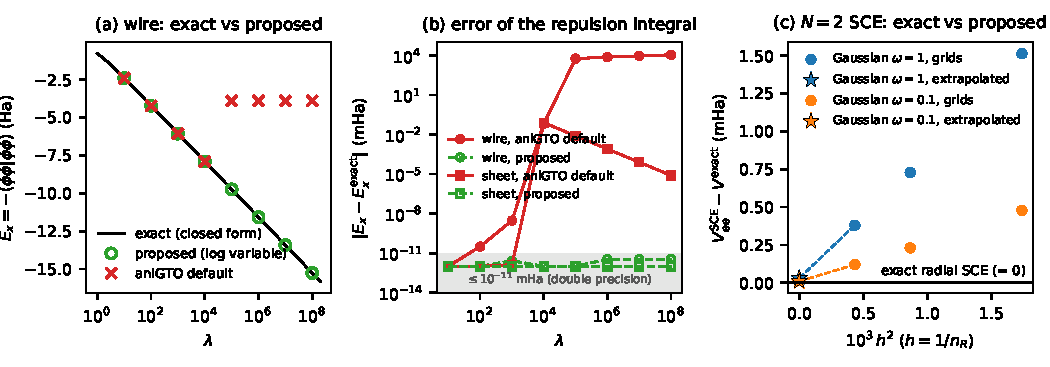
\includegraphics[width=\linewidth]{scan1d2d_dcscan_exact_vs_proposed.pdf}
\caption{Matching of exact references and proposed methods.  (a) Wire
  self-repulsion versus $\lambda$: closed form (line), logarithmic-variable
  quadrature (circles) and aniGTO default quadrature (crosses), which
  collapses to $-3.906$~Ha for $\lambda\ge10^5$.  (b) Absolute errors (mHa)
  for the wire and the sheet; the shaded band is the double-precision limit.
  (c) $N=2$ SCE energy of isotropic Gaussians: axisymmetric optimal-transport
  values on three grids (circles) against $h^2$, and the extrapolated values
  (stars), which coincide with the exact radial solution (zero line) to 0.03
  and 0.009~mHa.}
\label{fig:exact-vs-proposed}
\end{figure}

\subsection{Beyond the semilocal form}
\label{sec:beyond}
We tested two routes beyond the semilocal form on the same wires (SI,
Section~\href{si.pdf\#section.6}{S6}); our analysis shows that range-separated
hybrids do not help,
because 90--98\% of the wire exchange is short-range at the HSE06 screening
parameter.  First, a quasi-1D LDA built on the Kantorovich kernel $w_b$, with
$b$ taken from the density curvature, reproduces the wire logarithm exactly;
its error, $+120.2$~mHa for every $\lambda\ge100$, is a $\lambda$-independent
constant from the axial inhomogeneity, and a one-parameter 1D gradient
correction fitted on the Gaussian removes it there (0.03~mHa) but not on other
axial profiles.  Second, a local hybrid that mixes in exact exchange with the
iso-orbital weight $a=\tau_W/\tau$ is exact for $N=2$ (0.000~mHa at every
$\lambda$).  For $N=4$ and 6 wires built from the $s$, $p_z$ and $d_{zz}$
functions of the same aniGTO trap basis, with the exact exchange-energy
density from the same anisotropic integrals, its error falls from tens of mHa
at $\lambda\le100$ to $-0.10$ and $-0.30$~mHa (LH-DC-SCAN) at
$\lambda=10^4$, because $a\to1$ once the transverse kinetic energy dominates.
DC-SCAN alone, whose 1D branch was fixed on $N=2$, misses by $-0.44$ and
$-0.93$~Ha there.

\section{Conclusions}
\label{sec:conclusions}
In this study, we have shown that on one-orbital densities the SCAN indicator
$\alpha$ vanishes and cannot distinguish confinement geometries.  On exactly
solvable two-electron Gaussian densities this makes SCAN exchange diverge as
$\lambda^{1/2}$ under
wire confinement, instead of logarithmically, and converge to a sheet limit
8.9 times too negative; \novelty{applied to the infinite-barrier slab, the same analysis
reproduces the independent results of Constantin and of Kaplan, Wagle and Perdew
to 0.02\%.}  We have developed DC-SCAN, in which the log-density
curvature supplies the missing geometric information.  With two coefficients
fixed analytically on the Gaussian references, our DC-SCAN candidate captures
the exact wire logarithm
up to a finite-width offset of $-0.040$~Ha and reaches the exact sheet limit,
while leaving the uniform-gas and slowly varying limits of SCAN unchanged.
Our evaluation of the same functional inside aniGTO exposed two numerical
requirements: a logarithmic radial grid around the confinement axis for
Hessian-dependent functionals, and a logarithmic-variable repulsion integral
for exponent ratios beyond $10^8$.  We stress that these are fixed-density,
exchange-only results on one Gaussian profile per family.  Other confinement profiles,
three-dimensional norms (H, He, Ne, jellium), smooth regularization of $D$
and $\ln n$, the self-consistent potential (Appendix~\ref{app:scf}) and
correlation remain to be tested, and we will address them before DC-SCAN can be
considered a transferable functional.

\appendix

\refstepcounter{section}
\section*{Appendix~\thesection: Theory and Equations of DC-SCAN}
\addcontentsline{toc}{section}{Appendix~\thesection: Theory and Equations of DC-SCAN}
\label{app:theory}
\setcounter{equation}{0}
\renewcommand{\theequation}{A\arabic{equation}}
This appendix collects all definitions and derivations of the DC-SCAN
candidate; eqs~A1--A44 correspond one-to-one, in order, to Eqs.~(1)--(44) of
the DC-SCAN technical note (\texttt{reference/DC\_SCAN\_detailed\_theory\_results.pdf}).  Throughout, the Coulomb interaction is the three-dimensional
$1/r_{12}$ interaction and all coordinates are in bohr.

\subsection{Main working equations}
\begin{align}
E_x^{\mathrm{DC\text{-}SCAN}}[n]&=-C_x\int d^3r\,n^{4/3}(\mathbf r)\,
F_x^{\mathrm{DC\text{-}SCAN}}(s,\alpha,D,Z),
\label{eq:dc-E}\\
F_x^{\mathrm{DC\text{-}SCAN}}&=\bigl[1-\Omega(w_{2D}+w_{1D})\bigr]F_x^{\mathrm{SCAN}}(s,\alpha)
+\Omega\bigl[w_{2D}F_{2D}(s)+w_{1D}F_{1D}(s)\bigr],
\label{eq:dc-main}
\end{align}
where $C_x=\tfrac34(3/\pi)^{1/3}$, $F_{2D}(s)=0.65322589699\,(1+s^2)^{-1/4}$,
$F_{1D}(s)=\{3(1+s^2)\}^{-1}$, and $D$, $Z$, $w_j$ and $\Omega$ are defined
below.  These numerical coefficients follow from the chosen two-electron
Gaussian densities; they are not universal constants of an exact exchange
functional.

\subsection{SCAN exchange}
Standard SCAN exchange\cite{sun2015strongly} is
\begin{align}
E_x^{\mathrm{SCAN}}[n]&=-C_x\int n^{4/3}F_x^{\mathrm{SCAN}}(s,\alpha)\,d^3r,
\label{eq:dc-scanE}\\
s&=\frac{|\nabla n|}{2k_Fn},\qquad k_F=(3\pi^2n)^{1/3},
\label{eq:dc-s}\\
\alpha&=\frac{\tau-\tau_W}{\tau_{\mathrm{unif}}},\qquad
\tau_W=\frac{|\nabla n|^2}{8n},\qquad
\tau_{\mathrm{unif}}=\frac{3}{10}k_F^2n.
\label{eq:dc-alpha}
\end{align}
For a spin-unpolarized two-electron state with a single doubly occupied real
spatial orbital, $\tau=\tau_W$ and $\alpha=0$, irrespective of whether the
density is spherical, sheet-like or wire-like.  On this branch
\begin{equation}
F_x^{\mathrm{SCAN}}(s,0)=1.174\bigl[1-\exp(-4.9479/\sqrt s)\bigr]
\;\underset{s\to\infty}{\sim}\;5.8088346\,s^{-1/2}.
\label{eq:dc-scan0}
\end{equation}

\subsection{Exact two-electron reference densities}
The normalized reference families are
\begin{align}
n_\lambda^{\mathrm{sheet}}(x,y,z)&=\frac{2\lambda}{\pi^{3/2}}
\exp[-(x^2+y^2+\lambda^2z^2)],
\label{eq:dc-nsheet}\\
n_\lambda^{\mathrm{wire}}(x,y,z)&=\frac{2\lambda^2}{\pi^{3/2}}
\exp[-(\lambda^2(x^2+y^2)+z^2)],
\label{eq:dc-nwire}
\end{align}
with $\lambda\ge1$.  They integrate to $N=2$ and are each generated by one
real doubly occupied orbital, so $\alpha=0$ wherever $n>0$.  The
exchange-only exact reference is
\begin{equation}
E_x^{\mathrm{exact}}[n]=-\frac12E_H[n]
=-\frac14\iint\frac{n(\mathbf r)\,n(\mathbf r')}{|\mathbf r-\mathbf r'|}\,d^3r\,d^3r'.
\label{eq:dc-exact}
\end{equation}
Gaussian Coulomb integration (Appendix~\ref{app:coulomb}) gives, for
$\lambda>1$,
\begin{align}
E_x^{\mathrm{sheet,exact}}(\lambda)&=-\sqrt{\frac{2}{\pi}}\,
\frac{\lambda}{\sqrt{\lambda^2-1}}\,\arctan\sqrt{\lambda^2-1},
\label{eq:dc-exsheet}\\
E_x^{\mathrm{wire,exact}}(\lambda)&=-\sqrt{\frac{2}{\pi}}\,
\frac{\lambda}{\sqrt{\lambda^2-1}}\,\arcosh\lambda.
\label{eq:dc-exwire}
\end{align}
Both approach $-\sqrt{2/\pi}$~Ha as $\lambda\to1$.  Their strongly confined
limits differ:
\begin{align}
E_x^{\mathrm{sheet,exact}}(\lambda)&\longrightarrow-\sqrt{\frac{\pi}{2}}
\qquad(\lambda\to\infty),
\label{eq:dc-sheetlim}\\
E_x^{\mathrm{wire,exact}}(\lambda)&=-\sqrt{\frac{2}{\pi}}\,\ln(2\lambda)
+O\!\left(\frac{\ln\lambda}{\lambda^2}\right).
\label{eq:dc-wirelim}
\end{align}
Sheet compression gives a finite exchange energy with the 3D $1/r$
interaction; the zero-width wire retains a logarithmic Coulomb singularity.

\subsection{Why the SCAN branch fails on the wire}
At generic scaled positions the reduced gradient behaves as
\begin{equation}
s_{\mathrm{sheet}}\sim\lambda^{2/3},\qquad s_{\mathrm{wire}}\sim\lambda^{1/3},
\label{eq:dc-sscaling}
\end{equation}
and the exchange volume factors scale as $n^{4/3}d^3r\sim\lambda^{1/3}$ and
$\lambda^{2/3}$, respectively.  Inserting $F_x(s,0)\sim s^{-1/2}$ gives a
finite sheet limit but
\begin{equation}
E_x^{\mathrm{SCAN}}[n_\lambda^{\mathrm{wire}}]\sim-\mathrm{const}\cdot\lambda^{1/2},
\label{eq:dc-scanwire}
\end{equation}
rather than the logarithm of eq~\ref{eq:dc-wirelim}.

\subsection{Log-density curvature and geometry descriptors}
The symmetric log-density curvature tensor is
\begin{equation}
C_{ij}=-\frac12\partial_i\partial_j\ln n=-\frac{n_{ij}}{2n}+\frac{n_in_j}{2n^2},
\qquad n_i=\partial_in,\quad n_{ij}=\partial_i\partial_jn.
\label{eq:dc-C}
\end{equation}
For the two Gaussian families it is position independent,
\begin{equation}
C^{\mathrm{sheet}}=\mathrm{diag}(1,1,\lambda^2),\qquad
C^{\mathrm{wire}}=\mathrm{diag}(\lambda^2,\lambda^2,1).
\label{eq:dc-Cgauss}
\end{equation}
The directional effective-rank descriptor and the curvature scale are
\begin{equation}
D=\clip_{[1,3]}\!\left(\frac{|\nabla n|^2\,\mathrm{Tr}(C^2)}{(\nabla n)^TC^2(\nabla n)}\right),
\qquad Z=\frac{\sqrt{\mathrm{Tr}(C^2)}}{k_F^2},
\label{eq:dc-DZ}
\end{equation}
with $D=3$ where the denominator vanishes.  At generic points of the Gaussian
families
\begin{equation}
D\to1\ \text{(sheet)},\qquad D\to2\ \text{(wire)},\qquad D=3\ \text{(isotropic)}.
\label{eq:dc-Dlimits}
\end{equation}
Under uniform coordinate scaling $n_\gamma(\mathbf r)=\gamma^3n(\gamma\mathbf r)$,
$C\mapsto\gamma^2C$ and $k_F^2\mapsto\gamma^2k_F^2$ at scaled positions, so $D$
and $Z$ are dimensionless scale-invariant fields; both are rotational scalars.
For the hydrogenic density $n\propto e^{-2\zeta r}$, $C$ has zero radial
curvature and $\nabla n$ is radial, and the convention gives $D=3$.

\subsection{DC-SCAN enhancement factor}
\begin{align}
F_x^{\mathrm{DC\text{-}SCAN}}(s,\alpha,D,Z)&=\bigl[1-\Omega(s,Z)(w_{2D}+w_{1D})\bigr]F_x^{\mathrm{SCAN}}(s,\alpha)
\notag\\&\quad+\Omega(s,Z)\bigl[w_{2D}F_{2D}(s)+w_{1D}F_{1D}(s)\bigr],
\label{eq:dc-Fx}\\
F_{2D}(s)&=\frac{A_{2D}}{(1+s^2)^{1/4}},\qquad F_{1D}(s)=\frac{A_{1D}}{1+s^2},
\label{eq:dc-branches}\\
A_{2D}&=0.6532258969913366,\qquad A_{1D}=\frac13.
\label{eq:dc-A}
\end{align}
The geometry weights are built from the polynomials
\begin{align}
L_{2D}(D)&=\tfrac12(D-2)(D-3),\qquad L_{1D}(D)=(D-1)(3-D),
\label{eq:dc-L}\\
L_{3D}(D)&=\tfrac12(D-1)(D-2),\qquad
w_j(D)=\frac{L_j(D)^2}{L_{2D}^2+L_{1D}^2+L_{3D}^2}.
\label{eq:dc-w}
\end{align}
They satisfy $0\le w_j\le1$ and $w_{2D}+w_{1D}+w_{3D}=1$ and select the 2D, 1D
and unmodified SCAN branches at $D=1$, 2 and 3.  The activation switch is
\begin{equation}
\Omega(s,Z)=\frac{Z^3}{1+Z^3}\,\frac{s^8}{1+s^8};
\label{eq:dc-Omega}
\end{equation}
the exponents 3 and 8 are design choices, and no molecular or solid-state
data are fitted.  An equivalent form displays the convex mixture,
\begin{equation}
F_x^{\mathrm{DC\text{-}SCAN}}=(1-\Omega)F_x^{\mathrm{SCAN}}
+\Omega\bigl[w_{2D}F_{2D}+w_{1D}F_{1D}+w_{3D}F_x^{\mathrm{SCAN}}\bigr].
\label{eq:dc-convex}
\end{equation}
If the base SCAN enhancement obeys a pointwise upper bound, this form
preserves the bound provided each added branch obeys it; both branches have
maxima below 1.174.

\subsection{Analytic choice of the coefficients}
\paragraph{Sheet.}  Let $c=2/\pi^{3/2}$ and $K=(3\pi^2)^{1/3}$.  With
$u=x^2+y^2$ and $t=\lambda z$, the sheet has $n=\lambda c\exp(-u-t^2)$ and
\begin{equation}
s=\frac{\sqrt{u+\lambda^2t^2}}{Kn^{1/3}}\sim
\frac{\lambda^{2/3}|t|}{K[c\exp(-u-t^2)]^{1/3}}\qquad(t\ne0).
\label{eq:dc-ssheet}
\end{equation}
For $F_{2D}\sim A_{2D}s^{-1/2}$ the integrated exchange tends to
$-A_{2D}M_{2D}$, with
\begin{equation}
M_{2D}=C_x\sqrt K\,c^{3/2}\left(\frac{2\pi}{3}\right)
\left(\frac32\right)^{-1/4}\Gamma\!\left(\frac14\right)=1.918653475142493.
\label{eq:dc-M2D}
\end{equation}
Matching eq~\ref{eq:dc-sheetlim} fixes
\begin{equation}
A_{2D}=\frac{\sqrt{\pi/2}}{M_{2D}}=0.6532258969913366.
\label{eq:dc-A2D}
\end{equation}
The 2D Gaussian reference limit, including its coefficient, is thus imposed
analytically; it is not an exact result for an arbitrary 2D electron gas.

\paragraph{Wire.}  With $u=\lambda^2(x^2+y^2)$ and $t=z$,
$n=\lambda^2c\exp(-u-t^2)$ and
\begin{equation}
s\sim\frac{\lambda^{1/3}\sqrt u}{K[c\exp(-u-t^2)]^{1/3}}\qquad(u>0).
\label{eq:dc-swire}
\end{equation}
When $F_{1D}\sim A_{1D}/s^2$, the radial integral has a logarithmic region
$\lambda^{-2/3}\ll u\ll1$, in which $du/u$ supplies $\tfrac23\ln\lambda$, and
\begin{equation}
E_x^{1D}\sim-\underbrace{\left[\frac{2\pi}{3}C_xK^2c^2\sqrt{\frac{\pi}{2}}\right]}_{3\sqrt{2/\pi}}
A_{1D}\ln\lambda+O(1).
\label{eq:dc-E1D}
\end{equation}
Matching the exact coefficient $\sqrt{2/\pi}$ of eq~\ref{eq:dc-wirelim} gives
\begin{equation}
A_{1D}=\frac13.
\label{eq:dc-A1D}
\end{equation}
This fixes the coefficient of the logarithm, not the finite-width energy or
its $O(1)$ constant.

\subsection{Fixed-density quadrature}
In cylindrical coordinates and the transformed variables $u,t\ge0$ above,
\begin{equation}
E_x=-2\pi C_xc^{4/3}\lambda^{k/3}\int_0^\infty du\int_0^\infty dt\;
\exp\!\left[-\tfrac43(u+t^2)\right]F_x(s,\alpha=0,D,Z),
\label{eq:dc-quad}
\end{equation}
with $k=1$ for the sheet and $k=2$ for the wire.

\subsection{Self-consistent functional derivative}
\label{app:scf}
The energy density is
$e_x=-C_xn^{4/3}F_x^{\mathrm{DC\text{-}SCAN}}(n,\nabla n,\nabla\nabla n,\tau)$.
Its density-dependent Euler derivative is
\begin{equation}
v_x^{\mathrm{dens}}=\frac{\partial e_x}{\partial n}
-\partial_i\!\left(\frac{\partial e_x}{\partial n_i}\right)
+\partial_i\partial_j\!\left(\frac{\partial e_x}{\partial n_{ij}}\right).
\label{eq:dc-v}
\end{equation}
The $\tau$ dependence generates the usual generalized Kohn--Sham operator,
which acts on an orbital as
\begin{equation}
\tau_\sigma=\frac12\sum_{i\in\sigma}f_i|\nabla\phi_i|^2,\qquad
\hat V_{\tau,\sigma}\phi_{i\sigma}=-\frac12\nabla\cdot
\left[\frac{\partial e_x}{\partial\tau_\sigma}\nabla\phi_{i\sigma}\right].
\label{eq:dc-vtau}
\end{equation}
Exact exchange spin scaling defines the spin-dependent functional,
\begin{equation}
E_x[n_\uparrow,n_\downarrow]=\tfrac12E_x^{\mathrm{DC\text{-}SCAN}}[2n_\uparrow,2\tau_\uparrow]
+\tfrac12E_x^{\mathrm{DC\text{-}SCAN}}[2n_\downarrow,2\tau_\downarrow],
\label{eq:dc-spin}
\end{equation}
where the second argument is the kinetic-energy-density input of each
spin-channel evaluation.  The Hessian dependence introduces up to
fourth-order spatial derivatives into the local potential.

\subsection{Minimal-information variant}
To test whether the curvature magnitude $Z$ is needed, the same $D$ and
weights are kept and $\Omega(s,Z)$ is replaced by
\begin{equation}
\Omega_{\min}(s)=\frac{s^8}{1+s^8}.
\label{eq:dc-Omegamin}
\end{equation}

\subsection{Explicit SCAN exchange ingredients}
\begin{align}
F_x^{\mathrm{SCAN}}(s,\alpha)&=\bigl\{h_x^1(s,\alpha)+f_x(\alpha)\bigl[h_x^0-h_x^1(s,\alpha)\bigr]\bigr\}g_x(s),
\label{eq:dc-scanfull}\\
h_x^0&=1.174,\qquad g_x(s)=1-\exp(-a_1/\sqrt s),
\label{eq:dc-h0}\\
h_x^1(s,\alpha)&=1+k_1-\frac{k_1}{1+x(s,\alpha)/k_1},
\label{eq:dc-h1}\\
x(s,\alpha)&=\mu s^2\left[1+\frac{b_4s^2}{\mu}e^{-|b_4|s^2/\mu}\right]
+\left[b_1s^2+b_2(1-\alpha)e^{-b_3(1-\alpha)^2}\right]^2,
\label{eq:dc-x}\\
f_x(\alpha)&=\begin{cases}
\exp[-c_1\alpha/(1-\alpha)], & \alpha<1,\\
0, & \alpha=1,\\
-d_x\exp[c_2/(1-\alpha)], & \alpha>1,
\end{cases}
\label{eq:dc-fx}
\end{align}
with $a_1=4.9479$, $k_1=0.065$, $\mu=10/81$, $b_1\simeq0.1566$,
$b_2\simeq0.1208$, $b_3=0.5$, $b_4\simeq0.1218$, $c_1=0.667$, $c_2=0.8$ and
$d_x=1.24$; $g_x(0)=1$ by continuity.  The Gaussian tests use only
$\alpha=0$, on which eq~\ref{eq:dc-scan0} is exact.

\subsection{Gaussian Coulomb formulas}
\label{app:coulomb}
For an anisotropic Gaussian density
$n_A(\mathbf r)=2\sqrt{\det A}\,\pi^{-3/2}e^{-\mathbf r^TA\mathbf r}$ with $A>0$,
write
\begin{equation}
\frac{1}{r_{12}}=\frac{2}{\sqrt\pi}\int_0^\infty e^{-t^2r_{12}^2}\,dt.
\label{eq:dc-gausstrans}
\end{equation}
The difference of two independently distributed Gaussian positions has
covariance $A^{-1}$, giving
\begin{equation}
E_x[n_A]=-\frac{2}{\sqrt\pi}\int_0^\infty
\frac{\sqrt{\det A}}{\sqrt{\det(A+2t^2I)}}\,dt.
\label{eq:dc-ex44}
\end{equation}
With $A=\mathrm{diag}(1,1,\lambda^2)$ or $\mathrm{diag}(\lambda^2,\lambda^2,1)$
elementary integration yields eqs~\ref{eq:dc-exsheet} and \ref{eq:dc-exwire};
the $\lambda=1$ limit follows by continuity.

\refstepcounter{section}
\section*{Appendix~\thesection: Constraint Audit}
\addcontentsline{toc}{section}{Appendix~\thesection: Constraint Audit}
\label{app:constraints}
\renewcommand{\thetable}{B\arabic{table}}
\setcounter{table}{0}
\begin{table}[H]
\centering
\caption{Status of the DC-SCAN exchange construction.  ``Retained'' applies to
  the definitions and assumptions of Appendix~\ref{app:theory}, not to all
  SCAN exchange--correlation conditions.}
\label{tab:constraints}
\small
\begin{tabular}{@{}p{0.38\linewidth}p{0.56\linewidth}@{}}
\toprule
Property & Status / reason \\
\midrule
Uniform electron gas & Retained: $s=0$ implies $\Omega=0$, so $F_x=F_x^{\mathrm{SCAN}}=1$. \\
Uniform coordinate scaling & Retained: $s$, $\alpha$, $D$ and $Z$ are dimensionless under scaling. \\
Rotational invariance & Retained: tensor contractions are scalars. \\
Exchange spin scaling & Retained with eq~\ref{eq:dc-spin}. \\
Gradient expansion to fourth order & Retained in a smooth slowly varying limit: $\Omega=O(s^8)$. \\
Pointwise bound $F_x\le1.174$ & Retained if SCAN obeys it: both branches stay below 1.174 and eq~\ref{eq:dc-convex} is a convex mixture. \\
Hydrogenic exponential density & Unmodified through $D=3$; other atomic norms not established. \\
Gaussian sheet energy limit & Imposed analytically through $A_{2D}$; checked numerically. \\
Gaussian wire leading logarithm & Imposed analytically through $A_{1D}$; checked numerically. \\
Exact exchange for arbitrary 2D/1D densities & Not established; coefficients depend on the reference profiles. \\
Exchange hole, potential regularity, nonuniform scaling, all SCAN constraints & Not established. \\
\bottomrule
\end{tabular}
\end{table}
A local integral of finitely many density derivatives is additive for
disjoint supports, whereas the two-electron exchange $-E_H/2$ contains the
Coulomb cross term between separated lobes; exact exchange for all
two-electron densities therefore requires nonlocal information.  In practice
$\ln n$ and $C$ are ill-conditioned in low-density tails and the clipping of
$D$ must be replaced by a differentiable regularization before a
self-consistent potential can be used.

\begin{suppinfo}
Numerical protocol and convergence checks; exact-exchange cross-checks for the
wire and the sheet; local slopes and the finite-width offset on the wire;
aniGTO grid comparison; sheet asymptotics; PBE base and refit of the
activation scales; range separation, quasi-1D LDA/GGA and local hybrids;
figures of the wire and sheet benchmarks (PDF).
\end{suppinfo}

% compiled bibliography inlined; no BibTeX run needed
\providecommand{\latin}[1]{#1}
\makeatletter
\providecommand{\doi}
  {\begingroup\let\do\@makeother\dospecials
  \catcode`\{=1 \catcode`\}=2 \doi@aux}
\providecommand{\doi@aux}[1]{\endgroup\texttt{#1}}
\makeatother
\providecommand*\mcitethebibliography{\thebibliography}
\csname @ifundefined\endcsname{endmcitethebibliography}
  {\let\endmcitethebibliography\endthebibliography}{}
\begin{mcitethebibliography}{7}
\providecommand*\natexlab[1]{#1}
\providecommand*\mciteSetBstSublistMode[1]{}
\providecommand*\mciteSetBstMaxWidthForm[2]{}
\providecommand*\mciteBstWouldAddEndPuncttrue
  {\def\EndOfBibitem{\unskip.}}
\providecommand*\mciteBstWouldAddEndPunctfalse
  {\let\EndOfBibitem\relax}
\providecommand*\mciteSetBstMidEndSepPunct[3]{}
\providecommand*\mciteSetBstSublistLabelBeginEnd[3]{}
\providecommand*\EndOfBibitem{}
\mciteSetBstSublistMode{f}
\mciteSetBstMaxWidthForm{subitem}{(\alph{mcitesubitemcount})}
\mciteSetBstSublistLabelBeginEnd
  {\mcitemaxwidthsubitemform\space}
  {\relax}
  {\relax}

\bibitem[Sun \latin{et~al.}(2015)Sun, Ruzsinszky, and Perdew]{sun2015strongly}
Sun,~J.; Ruzsinszky,~A.; Perdew,~J.~P. Strongly constrained and appropriately
  normed semilocal density functional. \emph{Phys. Rev. Lett.} \textbf{2015},
  \emph{115}, 036402, DOI: \doi{10.1103/PhysRevLett.115.036402}\relax
\mciteBstWouldAddEndPuncttrue
\mciteSetBstMidEndSepPunct{\mcitedefaultmidpunct}
{\mcitedefaultendpunct}{\mcitedefaultseppunct}\relax
\EndOfBibitem
\bibitem[Constantin(2008)]{constantin2008dimensional}
Constantin,~L.~A. Dimensional crossover of the exchange-correlation energy at
  the semilocal level. \emph{Phys. Rev. B} \textbf{2008}, \emph{78}, 155106,
  DOI: \doi{10.1103/PhysRevB.78.155106}\relax
\mciteBstWouldAddEndPuncttrue
\mciteSetBstMidEndSepPunct{\mcitedefaultmidpunct}
{\mcitedefaultendpunct}{\mcitedefaultseppunct}\relax
\EndOfBibitem
\bibitem[Kaplan \latin{et~al.}(2018)Kaplan, Wagle, and
  Perdew]{kaplan2018collapse}
Kaplan,~A.~D.; Wagle,~K.; Perdew,~J.~P. Collapse of the electron gas from three
  to two dimensions in {Kohn-Sham} density functional theory. \emph{Phys. Rev.
  B} \textbf{2018}, \emph{98}, 085147, DOI:
  \doi{10.1103/PhysRevB.98.085147}\relax
\mciteBstWouldAddEndPuncttrue
\mciteSetBstMidEndSepPunct{\mcitedefaultmidpunct}
{\mcitedefaultendpunct}{\mcitedefaultseppunct}\relax
\EndOfBibitem
\bibitem[Horowitz \latin{et~al.}(2023)Horowitz, Proetto, and
  Pitarke]{horowitz2023collapsing}
Horowitz,~C.~M.; Proetto,~C.~R.; Pitarke,~J.~M. Construction of a semilocal
  exchange density functional from a three-dimensional electron gas collapsing
  to two dimensions. \emph{Phys. Rev. B} \textbf{2023}, \emph{108}, 115119,
  DOI: \doi{10.1103/PhysRevB.108.115119}\relax
\mciteBstWouldAddEndPuncttrue
\mciteSetBstMidEndSepPunct{\mcitedefaultmidpunct}
{\mcitedefaultendpunct}{\mcitedefaultseppunct}\relax
\EndOfBibitem
\bibitem[Dabbaghi \latin{et~al.}(2026)Dabbaghi, Garc{\'i}a~Lastra, and
  de~Silva]{dabbaghi2026hessian}
Dabbaghi,~P.; Garc{\'i}a~Lastra,~J.~M.; de~Silva,~P. Self-consistent
  Hessian-level meta-generalized gradient approximation. \emph{Phys. Rev. B}
  \textbf{2026}, DOI: \doi{10.1103/x4qn-mbr1}\relax
\mciteBstWouldAddEndPuncttrue
\mciteSetBstMidEndSepPunct{\mcitedefaultmidpunct}
{\mcitedefaultendpunct}{\mcitedefaultseppunct}\relax
\EndOfBibitem
\bibitem[Chirchir \latin{et~al.}(2026)Chirchir, Jana, and
  {'S}miga]{chirchir2026anigto}
Chirchir,~G.; Jana,~S.; {'S}miga,~S. An Anisotropic Gaussian Integral Package
  for Quasi-Dimensional Quantum-Chemical Simulations. 2026; Manuscript in
  preparation\relax
\mciteBstWouldAddEndPuncttrue
\mciteSetBstMidEndSepPunct{\mcitedefaultmidpunct}
{\mcitedefaultendpunct}{\mcitedefaultseppunct}\relax
\EndOfBibitem
\end{mcitethebibliography}


\end{document}
